\subsection{Model Problems from Verbal Instruction}

% add outline page with current section highlighted.
\begin{frame}{Outline}{ $ \null $ }
	%\tableofcontents[currentsection]
	\tableofcontents[currentsection,currentsubsection]
\end{frame}

\begin{frame}{The Spatial Hierarchy}{Related Work}

\begin{figure}
	\centering
	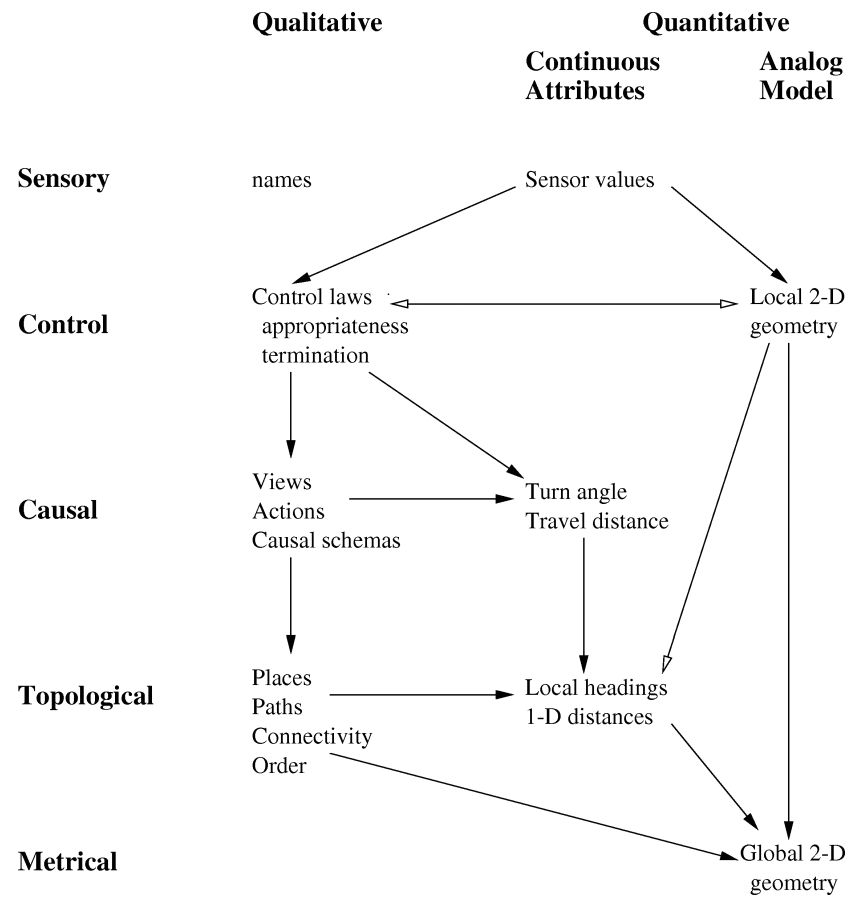
\includegraphics[width=.45\linewidth]{figure/semantic_hierarchy}
	\caption{ \tiny{ {\it Kuipers et al. } ``The spatial semantic hierarchy.'' Artificial intelligence 2000 } }
\end{figure}

\end{frame}

\begin{frame}{Spatial Description Clause}{Related Work}

\begin{figure}
	\centering
	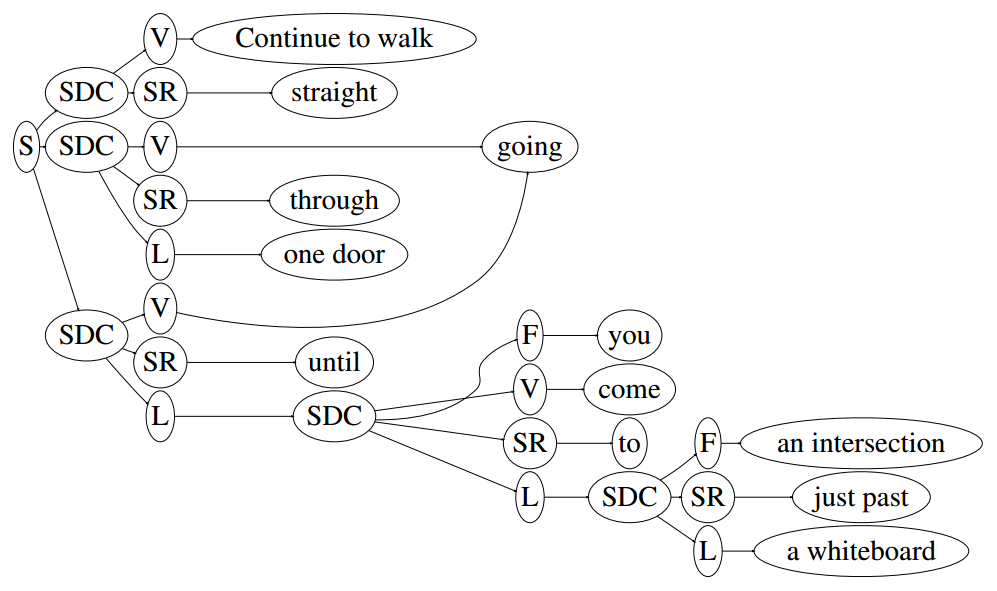
\includegraphics[width=.7\linewidth]{figure/spatial_description_clause}
	\caption{ \tiny{ {\it Kollar et al.} ``Toward understanding natural language directions.'' 5th ACM/IEEE International Conference on Human-Robot Interaction (HRI) 2010.} }
\end{figure}

\end{frame}

\begin{frame}{Tactical Behavior Specification}{Related Work}

\begin{figure}
	\centering
	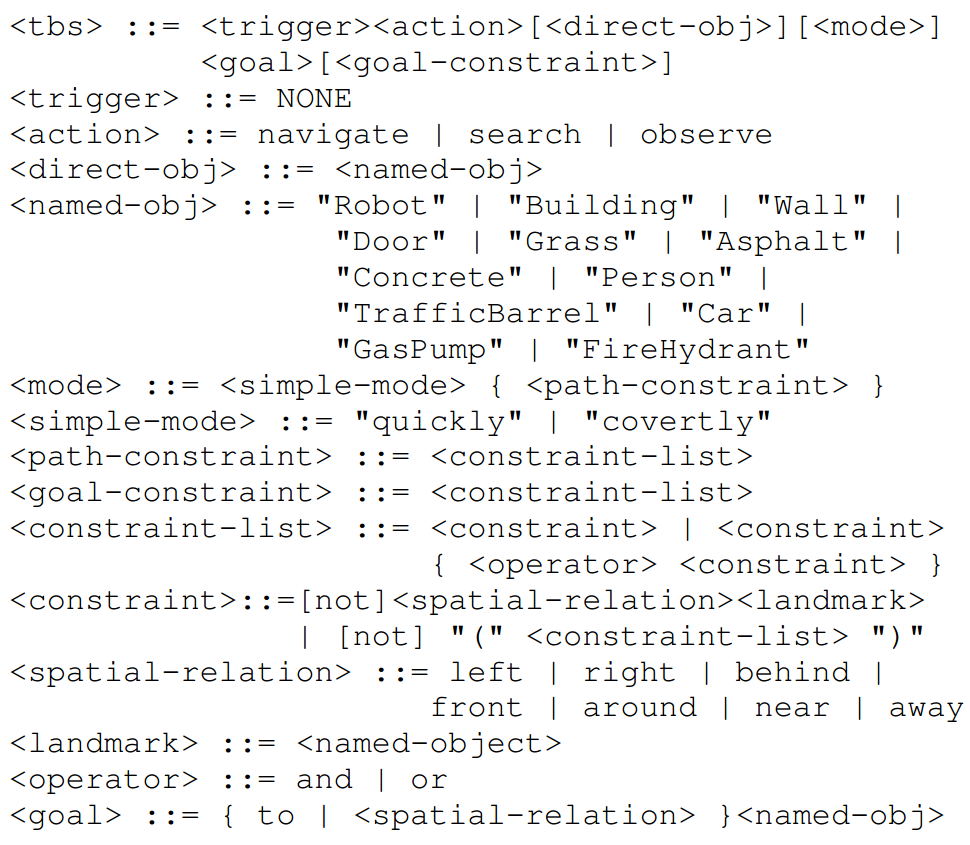
\includegraphics[width=.5\linewidth]{figure/tactical_behavior_specification}
	\caption{ \tiny{ {\it Boularias et al. } ``Grounding spatial relations for outdoor robot navigation.'' 2015 IEEE International Conference on Robotics and Automation (ICRA) 2015. } }
\end{figure}

\end{frame}

\begin{frame}{Inferring Information from Language Instructions}{Related Work}

\begin{figure}
	\centering
	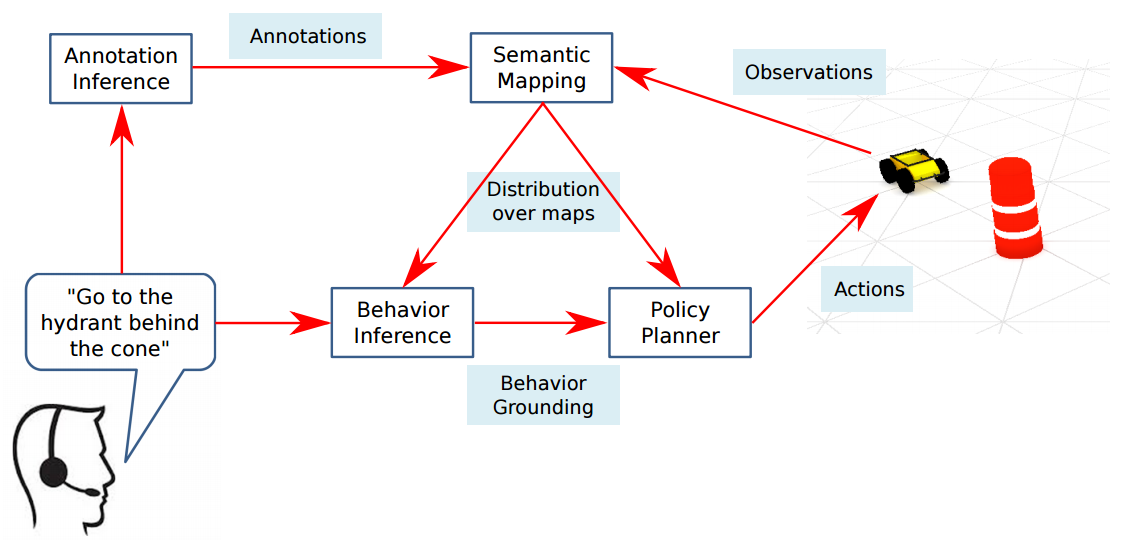
\includegraphics[width=.7\linewidth]{figure/inferring_information_from_language}
	\caption{ \tiny{ {\it Duvallet et al. } ``Inferring maps and behaviors from natural language instructions.'' International Symposium on Experimental Robotics (ISER)  2014. } }
\end{figure}

\end{frame}

\begin{frame}{Language Understanding}{Related Work}

{\bf G3 Model (Generalized Grounding Graph)\footnotemark }

\begin{figure}
	\centering
	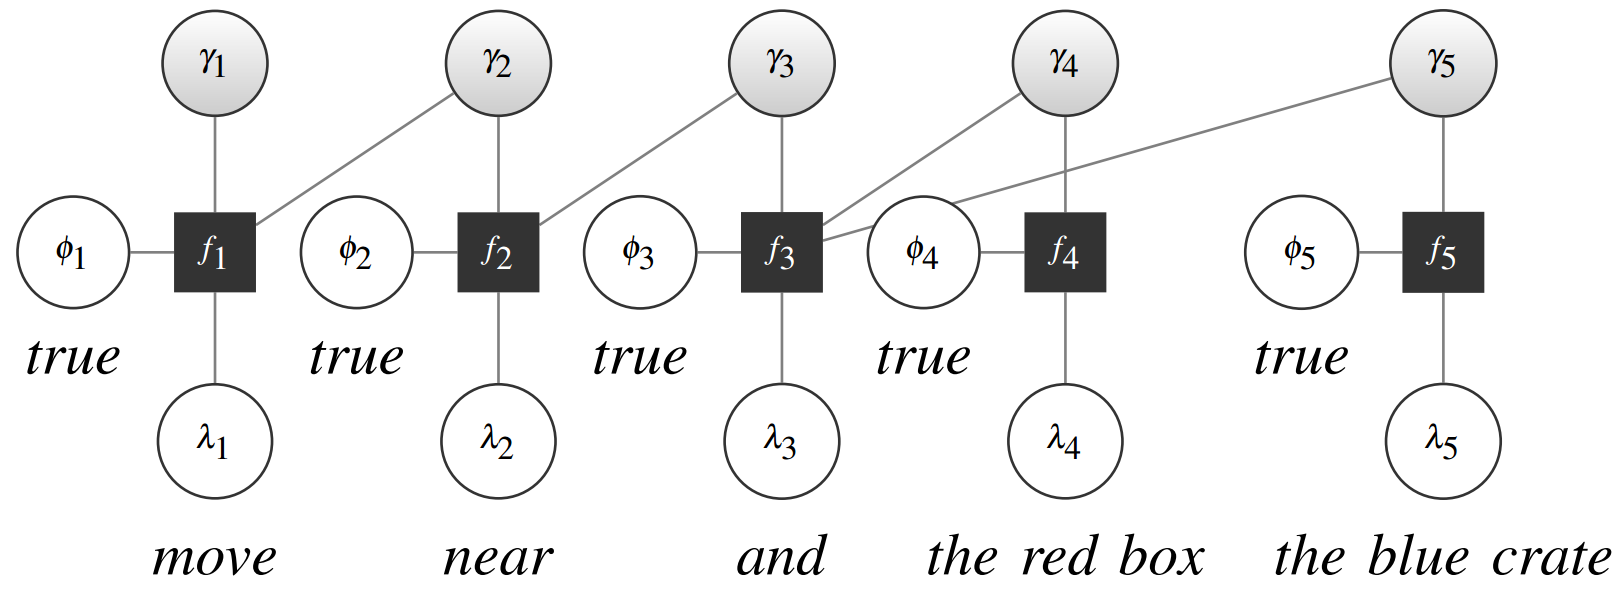
\includegraphics[width=.7\linewidth]{figure/G3}
	\caption{ \tiny{ {\it Howard et al.} ``A natural language planner interface for mobile manipulators.'' 2014 IEEE International Conference on Robotics and Automation (ICRA) 2014. } }
\end{figure}

\footnotetext[5]{\tiny {\it Tellex et al.} ``Understanding Natural Language Commands for Robotic Navigation and Mobile Manipulation.'' AAAI 2011.}

\end{frame}

\begin{frame}{Language Understanding}{Related Work}

{\bf DCG Model (Distributed Correspondence Graph)\footnotemark }

\begin{figure}
	\centering
	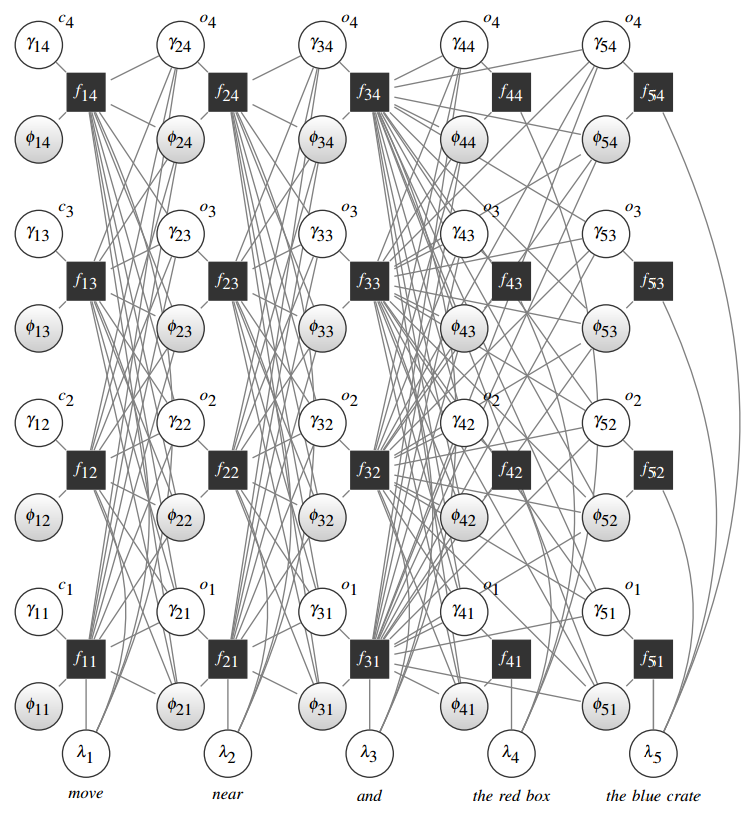
\includegraphics[width=.35\linewidth]{figure/DCG}
	\caption{ \tiny{ {\it Howard et al.} ``A natural language planner interface for mobile manipulators.'' 2014 IEEE International Conference on Robotics and Automation (ICRA) 2014. } }
\end{figure}

\footnotetext[6]{\tiny{ {\it Howard et al.} ``A natural language planner interface for mobile manipulators.'' 2014 IEEE International Conference on Robotics and Automation (ICRA) 2014. }}

\end{frame}

\begin{frame}{Language Understanding}{Related Work}

{\bf Hybrid G3-DCG Model }

\begin{figure}
	\centering
	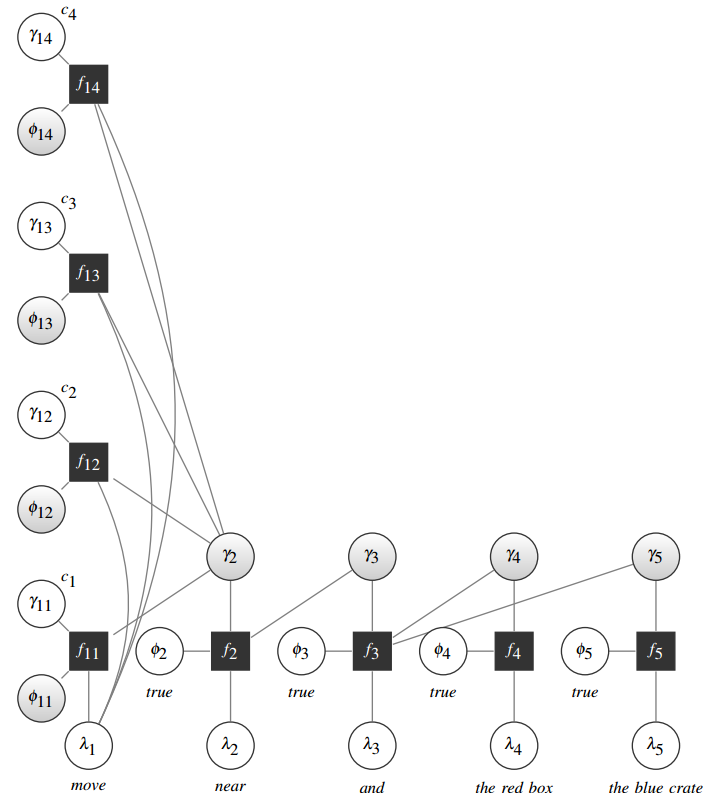
\includegraphics[width=.35\linewidth]{figure/hybrid_G3_DCG}
	\caption{ \tiny{ {\it Howard et al.} ``A natural language planner interface for mobile manipulators.'' 2014 IEEE International Conference on Robotics and Automation (ICRA) 2014. } }
\end{figure}

\end{frame}